\documentclass[11pt,aspectratio=169]{beamer}
\usetheme{Madrid}

% ======================= PACKAGES =======================
\usepackage{graphicx}
\usepackage{booktabs}
\usepackage{adjustbox}
\usepackage{multicol}
\usepackage{amsmath}
\usepackage{amssymb}
\usepackage{tikz}
\usetikzlibrary{arrows,shapes,positioning,shadows,trees}
\usepackage{listings}
\usepackage{xcolor}

% ======================= COLOR DEFINITIONS =======================
% Primary color scheme: Blue/Teal for Digital Finance
\definecolor{dfblue}{RGB}{0,102,204}
\definecolor{dfteal}{RGB}{0,153,153}
\definecolor{dfcyan}{RGB}{51,187,204}
\definecolor{dflightblue}{RGB}{153,204,255}
\definecolor{dflightblue2}{RGB}{173,214,255}
\definecolor{dflightblue3}{RGB}{193,224,255}
\definecolor{dflightblue4}{RGB}{213,234,255}

% Accent colors for finance applications
\definecolor{dfgreen}{RGB}{44, 160, 44}
\definecolor{dfred}{RGB}{214, 39, 40}
\definecolor{dforange}{RGB}{255, 127, 14}
\definecolor{dfgray}{RGB}{127, 127, 127}

% Utility colors
\definecolor{lightgray}{RGB}{240, 240, 240}
\definecolor{midgray}{RGB}{180, 180, 180}
\definecolor{codebg}{RGB}{245, 245, 245}

% ======================= THEME CUSTOMIZATION =======================
% Apply Digital Finance color scheme to Madrid theme
\setbeamercolor{palette primary}{bg=dflightblue3,fg=dfblue}
\setbeamercolor{palette secondary}{bg=dflightblue2,fg=dfblue}
\setbeamercolor{palette tertiary}{bg=dfteal,fg=white}
\setbeamercolor{palette quaternary}{bg=dfblue,fg=white}

\setbeamercolor{structure}{fg=dfblue}
\setbeamercolor{section in toc}{fg=dfblue}
\setbeamercolor{subsection in toc}{fg=dfteal}
\setbeamercolor{title}{fg=dfblue}
\setbeamercolor{frametitle}{fg=dfblue,bg=dflightblue3}
\setbeamercolor{block title}{bg=dflightblue2,fg=dfblue}
\setbeamercolor{block body}{bg=dflightblue4,fg=black}

% Remove navigation symbols for cleaner look
\setbeamertemplate{navigation symbols}{}

% Clean itemize/enumerate
\setbeamertemplate{itemize items}[circle]
\setbeamertemplate{enumerate items}[default]

% Margins for readability
\setbeamersize{text margin left=8mm,text margin right=8mm}

% ======================= LISTINGS CONFIGURATION =======================
% Python code style
\lstdefinestyle{pythonstyle}{
    language=Python,
    basicstyle=\ttfamily\footnotesize,
    keywordstyle=\color{dfblue}\bfseries,
    stringstyle=\color{dforange},
    commentstyle=\color{dfgray}\itshape,
    numberstyle=\tiny\color{dfgray},
    numbers=left,
    numbersep=5pt,
    backgroundcolor=\color{codebg},
    showspaces=false,
    showstringspaces=false,
    showtabs=false,
    frame=single,
    rulecolor=\color{midgray},
    tabsize=4,
    captionpos=b,
    breaklines=true,
    breakatwhitespace=false,
    escapeinside={(*@}{@*)},
    xleftmargin=10pt,
    xrightmargin=10pt
}

% Solidity code style
\lstdefinestyle{soliditystyle}{
    language=Java, % closest approximation
    basicstyle=\ttfamily\footnotesize,
    keywordstyle=\color{dfteal}\bfseries,
    stringstyle=\color{dforange},
    commentstyle=\color{dfgray}\itshape,
    numberstyle=\tiny\color{dfgray},
    numbers=left,
    numbersep=5pt,
    backgroundcolor=\color{codebg},
    showspaces=false,
    showstringspaces=false,
    showtabs=false,
    frame=single,
    rulecolor=\color{midgray},
    tabsize=2,
    captionpos=b,
    breaklines=true,
    breakatwhitespace=false,
    escapeinside={(*@}{@*)},
    xleftmargin=10pt,
    xrightmargin=10pt,
    morekeywords={pragma, contract, function, returns, public, private, view, pure, payable, address, uint256, mapping, event, modifier}
}

% Inline code command
\newcommand{\code}[1]{\texttt{\color{dfblue}#1}}

% ======================= CUSTOM COMMANDS =======================
% Bottom annotation (Madrid-style)
\newcommand{\bottomnote}[1]{%
\vfill
\vspace{-2mm}
\textcolor{dflightblue2}{\rule{\textwidth}{0.4pt}}
\vspace{1mm}
\footnotesize
\textbf{#1}
}

% Compact list spacing
\newcommand{\compactlist}{%
\setlength{\itemsep}{0pt}%
\setlength{\parskip}{0pt}%
\setlength{\parsep}{0pt}%
}

% Chart placeholder
\newcommand{\chartplaceholder}[2][5cm]{%
\begin{center}
\begin{adjustbox}{max width=0.95\textwidth, max height=#1}
\framebox[\textwidth][c]{%
\rule{0pt}{#1}%
\textcolor{midgray}{[#2]}%
}
\end{adjustbox}
\end{center}
}

% ======================= FINANCE NOTATION MACROS =======================
% Probability and statistics
\newcommand{\E}{\mathbb{E}} % Expected value
\newcommand{\Var}{\mathrm{Var}} % Variance
\newcommand{\Cov}{\mathrm{Cov}} % Covariance
\newcommand{\Prob}{\mathbb{P}} % Probability

% Distributions
\newcommand{\Normal}{\mathcal{N}} % Normal distribution
\newcommand{\Uniform}{\mathcal{U}} % Uniform distribution

% Returns and prices
\newcommand{\Ret}{R} % Return
\newcommand{\LogRet}{r} % Log return
\newcommand{\Price}{S} % Price/Stock price
\newcommand{\Strike}{K} % Strike price

% Options and derivatives
\newcommand{\CallPrice}{C} % Call option price
\newcommand{\PutPrice}{P} % Put option price
\newcommand{\Greeks}[1]{\mathit{#1}} % Greek letters

% Risk measures
\newcommand{\VaR}{\mathrm{VaR}} % Value at Risk
\newcommand{\CVaR}{\mathrm{CVaR}} % Conditional VaR
\newcommand{\Sharpe}{\mathrm{SR}} % Sharpe Ratio

% Time series
\newcommand{\AR}{\mathrm{AR}} % Autoregressive
\newcommand{\MA}{\mathrm{MA}} % Moving average
\newcommand{\GARCH}{\mathrm{GARCH}} % GARCH

% Blockchain/Crypto
\newcommand{\Hash}{\mathrm{Hash}} % Hash function
\newcommand{\Block}{\mathcal{B}} % Block
\newcommand{\Chain}{\mathcal{C}} % Chain

% Real numbers, integers
\newcommand{\R}{\mathbb{R}}
\newcommand{\Z}{\mathbb{Z}}
\newcommand{\N}{\mathbb{N}}

% ======================= TIKZ STYLES =======================
% Styles for finance-related diagrams
\tikzstyle{process} = [rectangle, minimum width=3cm, minimum height=1cm, text centered, draw=dfblue, fill=dflightblue4, thick]
\tikzstyle{decision} = [diamond, minimum width=3cm, minimum height=1cm, text centered, draw=dfteal, fill=dflightblue4, thick]
\tikzstyle{arrow} = [thick,->,>=stealth,color=dfblue]
\tikzstyle{blockchain} = [rectangle, rounded corners, minimum width=2.5cm, minimum height=1cm, text centered, draw=dfteal, fill=dflightblue3, thick]
\tikzstyle{transaction} = [circle, minimum size=0.8cm, text centered, draw=dforange, fill=dflightblue4, thick]

% ======================= FOOTER TEMPLATE =======================
\setbeamertemplate{footline}{
    \hbox{\begin{beamercolorbox}[wd=\paperwidth,ht=2.5ex,dp=1ex,leftskip=.5em,rightskip=.5em]{author in head/foot}
    \tiny
    \textbf{Digital Finance} \hfill
    Joerg Osterrieder \hfill
    \insertdate \hfill
    Page \insertframenumber{} / \inserttotalframenumber
    \end{beamercolorbox}}
}

% ======================= SECTION DIVIDER TEMPLATE =======================
\AtBeginSection[]{
\begin{frame}[plain]
\vfill
\centering
\begin{beamercolorbox}[sep=12pt,center]{title}
\usebeamerfont{title}\LARGE\insertsection\par
\end{beamercolorbox}
\vfill
\end{frame}
}


% ======================= DOCUMENT INFO =======================
\title{Topic 2.3: Data-Driven Finance}
\subtitle{Lending, Scoring, and Algorithmic Decision-Making}
\author{Joerg Osterrieder}
\institute{Digital Finance}
\date{}

\begin{document}

% ============================================================================
% SLIDE 1: Title
% ============================================================================
\begin{frame}[plain]
\titlepage
\end{frame}

% ============================================================================
% SLIDE 2: Learning Objectives
% ============================================================================
\begin{frame}{Learning Objectives}
\begin{block}{By the end of this topic, you will be able to:}
\begin{enumerate}
\item \textbf{Explain} how credit scoring works and why it matters for access to finance
\item \textbf{Identify} types of alternative data used in modern lending decisions
\item \textbf{Compare} traditional models with machine learning approaches at a conceptual level
\item \textbf{Recognize} sources of algorithmic bias and their real-world consequences
\item \textbf{Understand} why explainability is both a regulatory requirement and an ethical imperative
\item \textbf{Analyze} how data advantages create competitive moats in lending (NB04)
\end{enumerate}
\end{block}

\vspace{3mm}
\textbf{Key Competency}: Explain how data and algorithms are transforming lending decisions, and identify the ethical tensions that arise.

\bottomnote{Hands-on: Notebook NB04 -- Building a Credit Scoring Model}
\end{frame}

% ============================================================================
% SLIDE 3: Prerequisites -- Understanding Credit
% ============================================================================
\begin{frame}{Prerequisites: Understanding Credit}
\begin{columns}[T]
\begin{column}{0.5\textwidth}
\begin{alertblock}{Why Does Borrowing Exist?}
People need money \textit{now} for things they can afford over \textit{time}: a home, education, a car, or starting a business.
\end{alertblock}

\vspace{3mm}
\textbf{What is Credit?}
\begin{itemize}
\item A promise to repay later, usually with interest
\item Interest is the ``price'' of borrowing
\item The lender takes a risk; the borrower gains opportunity
\end{itemize}

\vspace{3mm}
\textbf{Types of Consumer Credit:}
\begin{itemize}
\item \textcolor{dfblue}{Revolving}: Credit cards, lines of credit (borrow and repay flexibly)
\item \textcolor{dfteal}{Installment}: Mortgages, auto loans, student loans (fixed repayment schedule)
\item \textcolor{dforange}{Point-of-sale}: Buy Now Pay Later (split purchases into payments)
\end{itemize}
\end{column}
\begin{column}{0.5\textwidth}
\begin{block}{Why Credit Matters}
\begin{itemize}
\item Enables major life purchases (home, education)
\item Smooths consumption over time
\item Fuels economic growth and entrepreneurship
\item Access to credit = economic opportunity
\end{itemize}
\end{block}

\vspace{3mm}
\begin{block}{The Insight}
Credit is so fundamental that being \textit{excluded} from it --- not being able to borrow at all --- is one of the biggest barriers to economic participation.
\end{block}
\end{column}
\end{columns}
\end{frame}

% ============================================================================
% SLIDE 4: The Core Problem of Lending
% ============================================================================
\begin{frame}{The Core Problem of Lending}
\begin{alertblock}{The Problem}
How does a lender decide whether to trust you with money they might never see again?
\end{alertblock}

\vspace{4mm}
\textbf{The Three Questions Every Lender Asks:}

\vspace{2mm}
\begin{columns}[T]
\begin{column}{0.32\textwidth}
\begin{block}{\textcolor{dfblue}{1. Willingness}}
\textit{Will} this person repay?
\begin{itemize}
\item Past payment behavior
\item Reliability track record
\item Character indicators
\end{itemize}
\end{block}
\end{column}
\begin{column}{0.32\textwidth}
\begin{block}{\textcolor{dfteal}{2. Capacity}}
\textit{Can} this person repay?
\begin{itemize}
\item Income and stability
\item Existing debts
\item Monthly obligations
\end{itemize}
\end{block}
\end{column}
\begin{column}{0.32\textwidth}
\begin{block}{\textcolor{dforange}{3. Collateral}}
What if they \textit{don't} repay?
\begin{itemize}
\item Assets the lender can claim
\item Secured vs. unsecured loans
\item Recovery value
\end{itemize}
\end{block}
\end{column}
\end{columns}

\vspace{4mm}
\begin{block}{The Insight}
Credit scoring automates these three judgments using data --- turning subjective assessments into systematic, scalable decisions.
\end{block}
\end{frame}

% ============================================================================
% SLIDE 5: Traditional Credit Scoring
% ============================================================================
\begin{frame}{Traditional Credit Scoring}
\begin{columns}[T]
\begin{column}{0.5\textwidth}
\begin{alertblock}{The Problem}
Lenders used to rely on personal relationships and gut feelings. How do you scale that to millions of applicants?
\end{alertblock}

\vspace{3mm}
\textbf{The Solution: Credit Scores}
\begin{itemize}
\item A credit score condenses your entire financial history into a \textbf{single number}
\item The number represents predicted creditworthiness
\item Scores span a range from \textbf{very poor to excellent}
\item Higher score = lower predicted risk = better loan terms
\end{itemize}

\vspace{3mm}
\textbf{Where Scores Are Used:}
\begin{itemize}
\item Loan approvals and interest rates
\item Credit card limits
\item Insurance pricing
\item Rental applications
\item Sometimes even employment screening
\end{itemize}
\end{column}
\begin{column}{0.5\textwidth}
\begin{block}{What Goes Into a Score}
Scores are built from categories of your financial behavior:
\begin{itemize}
\item How reliably you pay bills
\item How much debt you carry
\item How long you have been borrowing
\item How often you apply for new credit
\item What mix of credit types you use
\end{itemize}
\end{block}

\vspace{3mm}
\begin{block}{The Insight}
A single number determines the cost of many major life decisions --- your mortgage rate, your credit card limit, sometimes even whether you can rent an apartment.
\end{block}
\end{column}
\end{columns}
\end{frame}

% ============================================================================
% SLIDE 6: What Matters Most in a Credit Score
% ============================================================================
\begin{frame}{What Matters Most in a Credit Score}
\begin{alertblock}{The Problem}
Not all financial behaviors matter equally. What should a score emphasize?
\end{alertblock}

\vspace{3mm}
\textbf{Credit Score Components --- Ranked by Importance:}

\vspace{2mm}
\begin{center}
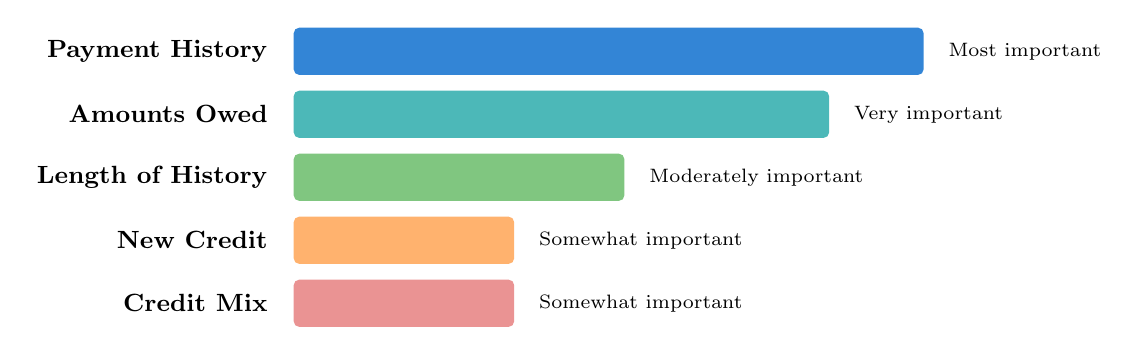
\begin{tikzpicture}[
    bar/.style={rectangle, rounded corners=2pt, minimum height=0.6cm, anchor=west, font=\small},
    label/.style={font=\small, anchor=east}
]
% Bars representing relative importance (qualitative, no percentages)
\node[bar, fill=dfblue!80, minimum width=8cm] at (0,3) {};
\node[label] at (-0.2,3) {\textbf{Payment History}};
\node[font=\scriptsize, anchor=west] at (8.2,3) {Most important};

\node[bar, fill=dfteal!70, minimum width=6.8cm] at (0,2.2) {};
\node[label] at (-0.2,2.2) {\textbf{Amounts Owed}};
\node[font=\scriptsize, anchor=west] at (7,2.2) {Very important};

\node[bar, fill=dfgreen!60, minimum width=4.2cm] at (0,1.4) {};
\node[label] at (-0.2,1.4) {\textbf{Length of History}};
\node[font=\scriptsize, anchor=west] at (4.4,1.4) {Moderately important};

\node[bar, fill=dforange!60, minimum width=2.8cm] at (0,0.6) {};
\node[label] at (-0.2,0.6) {\textbf{New Credit}};
\node[font=\scriptsize, anchor=west] at (3,0.6) {Somewhat important};

\node[bar, fill=dfred!50, minimum width=2.8cm] at (0,-0.2) {};
\node[label] at (-0.2,-0.2) {\textbf{Credit Mix}};
\node[font=\scriptsize, anchor=west] at (3,-0.2) {Somewhat important};
\end{tikzpicture}
\end{center}

\vspace{3mm}
\begin{block}{The Insight}
Your behavior with existing debt --- whether you pay on time and how much you owe --- matters far more than anything else. The most important factors are the ones you control through everyday financial discipline.
\end{block}
\end{frame}

% ============================================================================
% SLIDE 7: Who Gets Left Behind?
% ============================================================================
\begin{frame}{Who Gets Left Behind?}
\begin{columns}[T]
\begin{column}{0.5\textwidth}
\begin{alertblock}{The Problem}
What about people who have \textit{no} credit history at all?
\end{alertblock}

\vspace{3mm}
\textbf{``Credit Invisible'' --- No Score at All:}
\begin{itemize}
\item \textbf{Young adults}: Have not had time to build history
\item \textbf{Recent immigrants}: Foreign credit history does not transfer
\item \textbf{Cash-economy users}: Pay for everything without credit
\item \textbf{Divorced individuals}: Shared accounts removed
\item \textbf{Post-bankruptcy}: Wiped history, starting over
\end{itemize}

\vspace{3mm}
\textbf{The ``Thin File'' Problem:}\\
Some people have \textit{some} history, but not enough for a reliable score. They fall into a gray zone --- not scoreable, but not invisible either.
\end{column}
\begin{column}{0.5\textwidth}
\begin{block}{The Scale of the Problem}
Millions of people across every country are excluded from credit --- not because they are risky, but because the system has no data on them.
\end{block}

\vspace{3mm}
\textbf{The Catch-22:}
\begin{itemize}
\item You need credit to build a credit history
\item You need a credit history to get credit
\item This traps millions in a cycle of exclusion
\end{itemize}

\vspace{3mm}
\begin{block}{The Insight}
Millions of creditworthy people are excluded not because they \textit{cannot} repay, but because they lack traditional history. This is the opportunity that alternative data and FinTech try to address.
\end{block}
\end{column}
\end{columns}
\end{frame}

% ============================================================================
% SLIDE 8: The Credit Bureau System
% ============================================================================
\begin{frame}{The Credit Bureau System}
\begin{columns}[T]
\begin{column}{0.55\textwidth}
\begin{alertblock}{The Problem}
Where does all this credit data come from? Who collects and manages it?
\end{alertblock}

\vspace{3mm}
\textbf{What Credit Bureaus Do:}
\begin{itemize}
\item \textbf{Collect} credit data from banks, card companies, and lenders
\item \textbf{Maintain} individual credit files over time
\item \textbf{Sell} credit reports to lenders who request them
\item \textbf{Calculate} (or support calculation of) credit scores
\item \textbf{Resolve} consumer disputes about inaccuracies
\end{itemize}

\vspace{3mm}
\textbf{Bureau Data Sources:}
\begin{itemize}
\item Banks and credit unions
\item Credit card companies
\item Mortgage and auto lenders
\item Collection agencies
\item Public records (bankruptcies)
\end{itemize}
\end{column}
\begin{column}{0.45\textwidth}
\begin{block}{Key Concept}
Bureaus are \textbf{information intermediaries} --- they do \textit{not} make lending decisions. They provide the data infrastructure that lenders use to make their own decisions.
\end{block}

\vspace{3mm}
\textbf{How the System Works:}
\begin{enumerate}
\item Lenders report your payment behavior to bureaus
\item Bureaus compile your credit file
\item When you apply for credit, the new lender requests your report
\item The lender uses the report (and a score) to decide
\end{enumerate}

\vspace{3mm}
\begin{block}{The Insight}
The bureau system creates a shared record of trustworthiness --- but it only captures what lenders choose to report, leaving major gaps.
\end{block}
\end{column}
\end{columns}
\end{frame}

% ============================================================================
% SLIDE 9: Alternative Data -- A New Lens
% ============================================================================
\begin{frame}{Alternative Data: A New Lens}
\begin{alertblock}{The Problem}
What if we could assess creditworthiness using everyday financial behavior --- not just formal credit history?
\end{alertblock}

\vspace{3mm}
\begin{center}
\begin{tabular}{p{3.5cm}p{5cm}p{3cm}}
\toprule
\textbf{Data Type} & \textbf{What It Reveals} & \textbf{Who Benefits} \\
\midrule
Bank transactions & Cash flow patterns, income stability, spending habits & Thin-file borrowers \\
Rent payments & Reliability of regular payments & Young adults, renters \\
Utility bills & Consistent bill payment behavior & Cash-economy users \\
Employment/payroll & Job stability, income verification & Immigrants, gig workers \\
Education history & Future earning potential & Young graduates \\
Shopping behavior & Financial responsibility signals & Underbanked consumers \\
\bottomrule
\end{tabular}
\end{center}

\vspace{3mm}
\begin{block}{The Insight}
Alternative data can bring ``credit invisible'' people into the system --- scoring them on behaviors they already have, rather than formal credit products they lack.
\end{block}
\end{frame}

% ============================================================================
% SLIDE 10: Alternative Data -- Examples and Privacy
% ============================================================================
\begin{frame}{Alternative Data: Examples and Privacy}
\begin{columns}[T]
\begin{column}{0.5\textwidth}
\textbf{Bank Transaction Signals:}
\begin{itemize}
\item Income consistency and volatility
\item Ratio of rent to income
\item Frequency of overdrafts
\item Savings patterns over time
\item Recurring bill payment regularity
\end{itemize}

\vspace{3mm}
\textbf{Behavioral Data (More Controversial):}
\begin{itemize}
\item Time of day when applying
\item Device type and browser used
\item How form fields are completed
\item Typing speed and patterns
\item App usage patterns
\end{itemize}
\end{column}
\begin{column}{0.5\textwidth}
\begin{alertblock}{The Privacy Tension}
\textbf{More data} $\rightarrow$ better predictions $\rightarrow$ more inclusion

\vspace{2mm}
\textbf{More data} $\rightarrow$ deeper surveillance $\rightarrow$ privacy erosion

\vspace{2mm}
\textit{Where should the line be drawn?}
\end{alertblock}

\vspace{3mm}
\textbf{Key Questions:}
\begin{itemize}
\item Should your typing speed affect your loan rate?
\item Is using device data ``fair'' or invasive?
\item Who decides what data is appropriate?
\item Can consumers opt out of behavioral tracking?
\end{itemize}

\vspace{3mm}
\begin{block}{The Insight}
Every new data source that improves lending accuracy also raises a privacy question. There is no ``free'' improvement --- better predictions always come with ethical tradeoffs.
\end{block}
\end{column}
\end{columns}
\end{frame}

% ============================================================================
% SLIDE 11: Machine Learning in Credit
% ============================================================================
\begin{frame}{Machine Learning in Credit}
\begin{alertblock}{The Problem}
Can computers find patterns in data that humans miss?
\end{alertblock}

\vspace{3mm}
\begin{columns}[T]
\begin{column}{0.5\textwidth}
\textbf{Traditional Models:}
\begin{itemize}
\item Simple, well-understood rules
\item Easy to explain to regulators and applicants
\item Limited to relationships humans define
\item Proven track record over decades
\end{itemize}

\vspace{2mm}
\textit{Think of it as}: a carefully designed checklist where each item has a clear weight.
\end{column}
\begin{column}{0.5\textwidth}
\textbf{Machine Learning Models:}
\begin{itemize}
\item Can discover complex, hidden patterns
\item Handle hundreds of variables simultaneously
\item Significantly better at predicting defaults
\item Much harder to explain \textit{why} a decision was made
\end{itemize}

\vspace{2mm}
\textit{Think of it as}: a system that learns its own rules from the data --- powerful, but opaque.
\end{column}
\end{columns}

\vspace{4mm}
\begin{block}{The Insight}
Better accuracy comes at the cost of explainability. This is not just a technical annoyance --- it is a fundamental tension that shapes regulation, consumer trust, and business strategy in lending.
\end{block}
\end{frame}

% ============================================================================
% SLIDE 12: ML for Non-Programmers
% ============================================================================
\begin{frame}{Machine Learning for Non-Programmers}
\begin{columns}[T]
\begin{column}{0.5\textwidth}
\begin{alertblock}{The Problem}
What does ``machine learning'' actually mean in plain language?
\end{alertblock}

\vspace{3mm}
\begin{block}{Simple Definition}
Machine learning means \textbf{finding patterns in data} to make predictions about things you have not seen yet.
\end{block}

\vspace{3mm}
\textbf{The Checklist Analogy:}\\
Imagine a doctor's checklist for diagnosing illness:
\begin{itemize}
\item Some symptoms matter more than others
\item The checklist weighs each factor differently
\item The final diagnosis combines all factors
\end{itemize}

\vspace{2mm}
A traditional credit model works the same way --- a \textbf{sophisticated checklist} that weighs factors like payment history (most important), debt level (very important), and credit age (moderately important).
\end{column}
\begin{column}{0.5\textwidth}
\textbf{What ML Adds:}
\begin{itemize}
\item Traditional: Humans design the checklist
\item ML: The computer \textit{learns} its own checklist from data
\item ML can find patterns humans would never think to look for
\item But those patterns may be hard to explain
\end{itemize}

\vspace{3mm}
\textbf{Why Does This Matter for Lending?}
\begin{itemize}
\item Better patterns = fewer bad loans = lower costs
\item More variables considered = more people included
\item But: harder to explain = regulatory challenges
\end{itemize}

\vspace{3mm}
\begin{block}{The Insight}
The concept is simpler than the name suggests. Machine learning is just ``automated pattern-finding'' --- but the consequences of those patterns in lending are profound.
\end{block}
\end{column}
\end{columns}
\end{frame}

% ============================================================================
% SLIDE 13: The Credit Scoring Pipeline
% ============================================================================
\begin{frame}{The Credit Scoring Pipeline}
\begin{alertblock}{The Problem}
How does raw data become a lending decision?
\end{alertblock}

\vspace{3mm}
\begin{center}
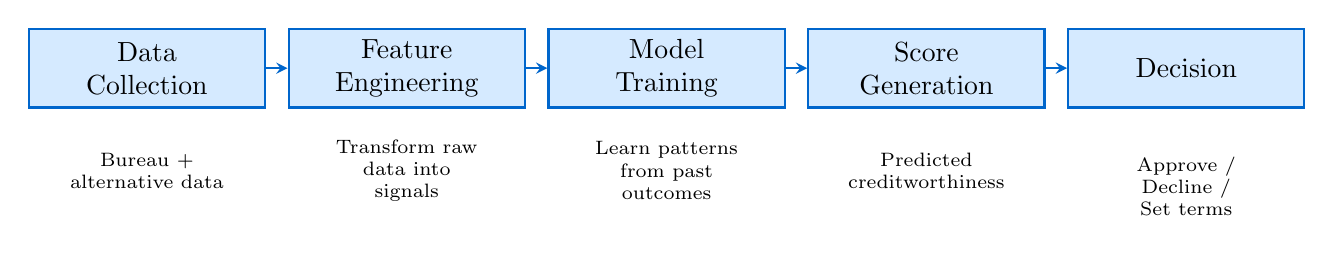
\begin{tikzpicture}[node distance=1.8cm]
% Pipeline nodes
\node (data) [process, align=center] {Data\\Collection};
\node (feature) [process, align=center, right of=data, xshift=1.5cm] {Feature\\Engineering};
\node (model) [process, align=center, right of=feature, xshift=1.5cm] {Model\\Training};
\node (score) [process, align=center, right of=model, xshift=1.5cm] {Score\\Generation};
\node (decision) [process, right of=score, xshift=1.5cm] {Decision};

% Arrows
\draw[arrow] (data) -- (feature);
\draw[arrow] (feature) -- (model);
\draw[arrow] (model) -- (score);
\draw[arrow] (score) -- (decision);

% Labels below
\node[below of=data, yshift=0.5cm, font=\scriptsize, text width=2cm, align=center] {Bureau +\\alternative data};
\node[below of=feature, yshift=0.5cm, font=\scriptsize, text width=2cm, align=center] {Transform raw\\data into signals};
\node[below of=model, yshift=0.5cm, font=\scriptsize, text width=2cm, align=center] {Learn patterns\\from past outcomes};
\node[below of=score, yshift=0.5cm, font=\scriptsize, text width=2cm, align=center] {Predicted\\creditworthiness};
\node[below of=decision, yshift=0.3cm, font=\scriptsize, text width=2cm, align=center] {Approve /\\Decline /\\Set terms};
\end{tikzpicture}
\end{center}

\vspace{3mm}
\textbf{Key Decisions at Each Stage:}
\begin{itemize}
\item \textbf{Data}: What sources? What are the privacy implications?
\item \textbf{Features}: What transformations? What should we exclude?
\item \textbf{Model}: How much accuracy vs. how much explainability?
\item \textbf{Decision}: Where do we set the approval threshold? When does a human review?
\end{itemize}

\vspace{2mm}
\begin{block}{The Insight}
Bias can enter at \textit{every} stage of this pipeline --- not just in the model itself, but in which data is collected, how features are designed, and where thresholds are set.
\end{block}
\end{frame}

% ============================================================================
% SLIDE 14: Feature Engineering
% ============================================================================
\begin{frame}[fragile]{Feature Engineering: From Raw Data to Useful Signals}
\begin{alertblock}{The Problem}
Raw data is messy. How do we turn it into inputs a model can use?
\end{alertblock}

\vspace{2mm}
\textbf{The Concept:} Feature engineering means creating meaningful signals from raw data. It is often the most important step in the pipeline --- a great feature matters more than a fancy algorithm.

\vspace{2mm}
\textbf{Conceptual Example --- Turning Transactions into Signals:}
\begin{lstlisting}[style=pythonstyle, basicstyle=\ttfamily\scriptsize]
# Raw data: a list of bank transactions (dates, amounts, categories)

# Engineered features (signals the model uses):
#   income_stability   = how consistent is monthly income?
#   spending_ratio     = spending relative to income
#   overdraft_frequency = how often does the account go negative?
#   bill_regularity    = are recurring bills paid on time?
#   savings_trend      = is the balance growing or shrinking?
\end{lstlisting}

\vspace{2mm}
\textbf{Why It Matters:}
\begin{itemize}
\item The \textit{same raw data} can produce very different features depending on design choices
\item Feature choices embed human assumptions about what matters
\item Poorly chosen features can introduce bias even from ``neutral'' data
\end{itemize}

\bottomnote{Notebook NB04: Engineer features from transaction data and see how they affect predictions}
\end{frame}

% ============================================================================
% SLIDE 15: Overfitting -- When Models Go Wrong
% ============================================================================
\begin{frame}{When Models Go Wrong: Overfitting}
\begin{columns}[T]
\begin{column}{0.5\textwidth}
\begin{alertblock}{The Problem}
What if a model memorizes the data instead of learning general patterns?
\end{alertblock}

\vspace{3mm}
\textbf{The Exam Analogy:}\\
Imagine studying for an exam by memorizing every answer from last year's test:
\begin{itemize}
\item You ace the practice test perfectly
\item But you fail the \textit{real} exam because the questions are different
\item You memorized answers instead of understanding concepts
\end{itemize}

\vspace{3mm}
\textbf{In Credit Scoring:}
\begin{itemize}
\item A model might learn: ``everyone from a certain area defaults''
\item In reality, that was just coincidence in the training data
\item New applicants from that area are unfairly rejected
\end{itemize}
\end{column}
\begin{column}{0.5\textwidth}
\begin{block}{The Solution: Training and Testing Split}
Hide some data from the model, then test it on data it has never seen.
\end{block}

\vspace{3mm}
\textbf{How It Works:}
\begin{enumerate}
\item Split data: most for training, some held back for testing
\item Train the model using only the training portion
\item Test the model on the held-back data
\item If test performance is similar to training: the model learned real patterns
\item If test performance is much worse: the model overfitted
\end{enumerate}

\vspace{3mm}
\begin{block}{The Insight}
Always test on data the model has never seen. A model that looks perfect on training data but fails on new data is worse than useless --- it gives false confidence.
\end{block}
\end{column}
\end{columns}
\end{frame}

% ============================================================================
% SLIDE 16: Algorithmic Bias -- The Dark Side
% ============================================================================
\begin{frame}{Algorithmic Bias: The Dark Side}
\begin{columns}[T]
\begin{column}{0.5\textwidth}
\begin{alertblock}{The Problem}
Can a ``neutral'' algorithm discriminate?
\end{alertblock}

\vspace{3mm}
\textbf{Sources of Bias:}
\begin{enumerate}
\item \textbf{Historical data bias}:\\
If past lending was discriminatory, the data reflects those patterns --- and the model learns to repeat them
\item \textbf{Proxy variables}:\\
Features like location or school can correlate with race or socioeconomic status
\item \textbf{Sample bias}:\\
Training only on existing customers misses the people who were already excluded
\item \textbf{Feature selection bias}:\\
Human choices about what data to include embed assumptions
\end{enumerate}
\end{column}
\begin{column}{0.5\textwidth}
\textbf{Real-World Example:}
\begin{itemize}
\item A major technology company launched a credit card
\item An algorithm set credit limits for applicants
\item People in the same household, with shared finances, received \textbf{dramatically different credit limits}
\item The algorithm could not explain why
\item A regulatory investigation followed
\end{itemize}

\vspace{3mm}
\textbf{Fairness Concepts:}
\begin{itemize}
\item \textbf{Demographic parity}: Approval rates similar across groups
\item \textbf{Equalized odds}: Error rates similar across groups
\item \textbf{Calibration}: Predictions equally accurate for all groups
\end{itemize}

\vspace{2mm}
\begin{block}{The Insight}
Bias in the data means bias in the decisions. Good intentions do not prevent harmful outcomes --- you must actively test for and mitigate bias.
\end{block}
\end{column}
\end{columns}
\end{frame}

% ============================================================================
% SLIDE 17: Proxy Variables and Disparate Impact
% ============================================================================
\begin{frame}{Proxy Variables and Disparate Impact}
\begin{columns}[T]
\begin{column}{0.5\textwidth}
\begin{alertblock}{The Problem}
What if a ``neutral'' feature --- like your home address --- effectively codes for race?
\end{alertblock}

\vspace{3mm}
\textbf{What is Disparate Impact?}
\begin{itemize}
\item A policy that \textit{appears} neutral on its face
\item But disproportionately harms a protected group
\item Even without any discriminatory \textit{intent}
\item Still illegal under fair lending laws in many jurisdictions
\end{itemize}

\vspace{3mm}
\textbf{Common Proxy Variables:}
\begin{itemize}
\item \textbf{Location} $\rightarrow$ can correlate with race (historical residential segregation)
\item \textbf{Name patterns} $\rightarrow$ can correlate with ethnicity
\item \textbf{School attended} $\rightarrow$ can correlate with socioeconomic status
\item \textbf{Occupation type} $\rightarrow$ can correlate with gender
\end{itemize}
\end{column}
\begin{column}{0.5\textwidth}
\begin{block}{Historical Context: Redlining}
\textbf{Redlining} was the historical practice of refusing loans to people in certain neighborhoods, often based on race. Though outlawed, its effects persist in data: neighborhoods that were ``redlined'' decades ago still show different economic patterns today.
\end{block}

\vspace{3mm}
\textbf{The Challenge for Algorithms:}
\begin{itemize}
\item Even if race is \textit{not} a feature, the model can learn to discriminate through proxies
\item Removing a proxy may reduce accuracy
\item Multiple proxies can combine to reconstruct protected attributes
\end{itemize}

\vspace{3mm}
\begin{block}{The Insight}
Even without explicit discrimination, algorithms can reproduce historical inequity. The question is not just ``is race in the model?'' but ``does the model \textit{behave differently} across racial groups?''
\end{block}
\end{column}
\end{columns}
\end{frame}

% ============================================================================
% SLIDE 18: Explainability -- The Right to Know Why
% ============================================================================
\begin{frame}{Explainability: The Right to Know Why}
\begin{columns}[T]
\begin{column}{0.5\textwidth}
\begin{alertblock}{The Problem}
If a machine denies you a loan, who explains why?
\end{alertblock}

\vspace{3mm}
\textbf{Why Explainability Matters:}
\begin{itemize}
\item \textbf{Regulatory requirement}: In many jurisdictions, lenders \textit{must} tell you why you were declined (``adverse action notice'')
\item \textbf{Consumer trust}: People need to understand decisions that affect their lives
\item \textbf{Model debugging}: Developers need to find and fix errors
\item \textbf{Fairness auditing}: Regulators need to verify the model is not discriminating
\end{itemize}

\vspace{3mm}
\textbf{What an Adverse Action Notice Looks Like:}\\
\textit{``Your application was declined because of: high debt relative to income, short credit history, and a recent late payment.''}
\end{column}
\begin{column}{0.5\textwidth}
\textbf{Explainability Techniques (Conceptual):}
\begin{itemize}
\item \textbf{Feature importance}: Which inputs matter most \textit{overall}?
\item \textbf{SHAP values}: How much did each input push \textit{this specific} decision up or down?
\item \textbf{Partial dependence}: How does changing one input affect the output?
\end{itemize}

\vspace{3mm}
\textbf{SHAP in Plain Language:}\\
Imagine you are splitting a restaurant bill fairly. SHAP assigns each feature its ``fair share'' of the prediction --- showing exactly which factors helped and which hurt.

\vspace{3mm}
\begin{block}{The Insight}
Explainability is both a regulatory requirement and an ethical imperative. Consumers deserve to understand the decisions that shape their financial lives --- and to have a path to challenge those decisions.
\end{block}
\end{column}
\end{columns}
\end{frame}

% ============================================================================
% SLIDE 19: Beyond Credit -- Algorithms Everywhere
% ============================================================================
\begin{frame}{Beyond Credit: Algorithms Everywhere in Finance}
\begin{alertblock}{The Problem}
Credit scoring was just the beginning. Where else are algorithms making financial decisions about you?
\end{alertblock}

\vspace{3mm}
\begin{columns}[T]
\begin{column}{0.5\textwidth}
\textbf{Insurance (Insurtech):}
\begin{itemize}
\item Driving behavior from telematics devices
\item Home sensor data from IoT devices
\item Claims fraud detection
\item Personalized, dynamic pricing
\end{itemize}

\vspace{3mm}
\textbf{Investment (Robo-Advisors):}
\begin{itemize}
\item Algorithmic risk profiling
\item Automated portfolio rebalancing
\item Tax-optimization strategies
\item Goal-based financial planning
\end{itemize}
\end{column}
\begin{column}{0.5\textwidth}
\textbf{Fraud Detection:}
\begin{itemize}
\item Real-time transaction scoring
\item Behavioral biometrics (how you hold your phone)
\item Device fingerprinting
\item Network analysis of suspicious patterns
\end{itemize}

\vspace{3mm}
\textbf{Identity Verification (KYC):}
\begin{itemize}
\item Automated document analysis
\item Facial recognition matching
\item Sanctions and watchlist screening
\item Suspicious activity pattern detection
\end{itemize}
\end{column}
\end{columns}

\vspace{3mm}
\begin{block}{The Insight}
Data and algorithms are replacing human judgment across \textit{all} of finance --- not just lending. The same tensions (accuracy vs. fairness, automation vs. explainability) apply everywhere.
\end{block}
\end{frame}

% ============================================================================
% SLIDE 20: The Data Flywheel
% ============================================================================
\begin{frame}{The Data Flywheel}
\begin{alertblock}{The Problem}
Why do data-rich companies keep getting stronger while newcomers struggle to compete?
\end{alertblock}

\vspace{3mm}
\begin{center}
\begin{tikzpicture}[node distance=2.5cm]
% Circular nodes
\node (more_data) [blockchain] {More Data};
\node (better_models) [blockchain, right of=more_data, xshift=2cm] {Better Models};
\node (better_decisions) [blockchain, below of=better_models] {Better Decisions};
\node (more_customers) [blockchain, left of=better_decisions, xshift=-2cm] {More Customers};

% Circular arrows
\draw[arrow, bend left=20] (more_data) to (better_models);
\draw[arrow, bend left=20] (better_models) to (better_decisions);
\draw[arrow, bend left=20] (better_decisions) to (more_customers);
\draw[arrow, bend left=20] (more_customers) to (more_data);

% Center label
\node at ($(more_data)!0.5!(better_decisions)$) {\textbf{Data Flywheel}};
\end{tikzpicture}
\end{center}

\vspace{3mm}
\begin{columns}[T]
\begin{column}{0.5\textwidth}
\textbf{How It Works:}
\begin{itemize}
\item More data improves model accuracy
\item Better models make better lending decisions
\item Better decisions attract more customers
\item More customers generate more data
\item The cycle \textit{compounds} over time
\end{itemize}
\end{column}
\begin{column}{0.5\textwidth}
\begin{block}{The Insight}
First-mover advantage in data creates a compounding moat. Incumbents have more historical data; newer entrants often have more \textit{diverse} data. The winner is whoever spins the flywheel fastest.
\end{block}
\end{column}
\end{columns}
\end{frame}

% ============================================================================
% SLIDE 21: Hands-On -- NB04
% ============================================================================
\begin{frame}{Hands-On: Notebook NB04 -- Credit Scoring Model}
\begin{block}{Exercise Overview}
In this notebook, you will walk through the entire credit scoring pipeline:
\begin{enumerate}
\item \textbf{Explore} a credit dataset and understand its structure
\item \textbf{Engineer features} from raw data to create predictive signals
\item \textbf{Build models} --- both a simple traditional model and a more complex one
\item \textbf{Compare} accuracy and interpretability between the two approaches
\item \textbf{Explain predictions} using feature importance and SHAP concepts
\item \textbf{Test for bias} across demographic groups
\end{enumerate}
\end{block}

\vspace{4mm}
\textbf{What You Will Learn:}
\begin{itemize}
\item How the accuracy-explainability tradeoff works in practice
\item Why feature engineering choices matter as much as model selection
\item How to probe models for potential algorithmic bias
\item The difference between a model that ranks well and one that predicts accurately
\end{itemize}

\vspace{3mm}
\bottomnote{No programming experience required --- the notebook guides you step by step}
\end{frame}

% ============================================================================
% SLIDE 22: Discussion -- Ethics of Algorithmic Lending
% ============================================================================
\begin{frame}{Discussion: The Ethics of Algorithmic Lending}
\begin{columns}[T]
\begin{column}{0.5\textwidth}
\textbf{Arguments FOR ML-Based Scoring:}
\begin{itemize}
\item More accurate models mean fewer bad loans, which can mean lower interest rates for everyone
\item Alternative data brings in people traditional scoring excludes
\item Algorithms are consistent --- they do not have ``bad days'' or personal prejudices
\item Faster decisions improve access to credit
\end{itemize}

\vspace{3mm}
\textbf{Arguments AGAINST:}
\begin{itemize}
\item Historical bias gets encoded and automated at scale
\item Lack of transparency is fundamentally unfair
\item Alternative data raises serious privacy concerns
\item Algorithmic errors are harder to detect and contest
\end{itemize}
\end{column}
\begin{column}{0.5\textwidth}
\begin{alertblock}{Discussion Questions}
\begin{enumerate}
\item Should lenders be allowed to use social media data in credit decisions?
\item Is it fair to use education level as a factor in lending?
\item Should all lending algorithms be required to be fully explainable?
\item If an algorithm discriminates unintentionally, who bears responsibility --- the developer, the lender, or the regulator?
\end{enumerate}
\end{alertblock}

\vspace{3mm}
\textbf{Think About:}\\
\textit{Is a biased algorithm better or worse than a biased human loan officer? Why?}
\end{column}
\end{columns}
\end{frame}

% ============================================================================
% SLIDE 23: Executive Summary
% ============================================================================
\begin{frame}{Executive Summary: Key Takeaways}
\begin{block}{Five Things to Remember from This Topic}
\begin{enumerate}
\item \textbf{Traditional scoring leaves people behind}: Credit scores are powerful but exclude millions of creditworthy people who lack formal credit history
\item \textbf{Alternative data expands access}: Bank transactions, rent payments, and employment data can bring excluded people into the credit system
\item \textbf{ML improves accuracy but reduces transparency}: Machine learning finds patterns humans miss, but creates ``black box'' challenges for regulators and consumers
\item \textbf{Bias is real and requires active mitigation}: Historical discrimination gets encoded in data; proxy variables can circumvent legal protections; good intentions alone do not prevent harm
\item \textbf{Explainability is non-negotiable}: Consumers have a right to know why they were denied credit --- this is both a legal requirement and an ethical imperative
\end{enumerate}
\end{block}

\vspace{3mm}
\textbf{Bottom Line}: Data-driven finance creates enormous opportunities for financial inclusion, but requires constant vigilance around fairness, transparency, and accountability.
\end{frame}

% ============================================================================
% SLIDE 24: Concept Map
% ============================================================================
\begin{frame}{Concept Map: Data-Driven Finance}
\begin{center}
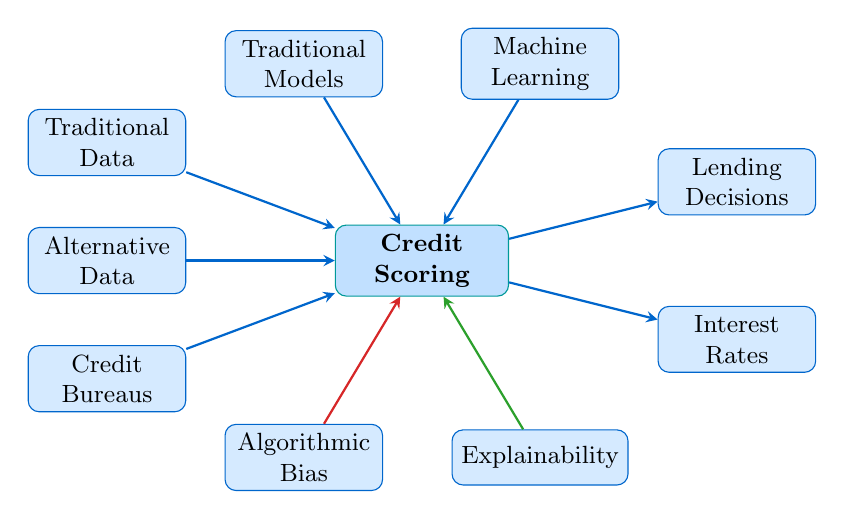
\begin{tikzpicture}[
    node distance=1.5cm,
    every node/.style={font=\small},
    box/.style={rectangle, rounded corners, draw=dfblue, fill=dflightblue4, minimum width=2cm, minimum height=0.7cm, align=center},
    bigbox/.style={rectangle, rounded corners, draw=dfteal, fill=dflightblue3, minimum width=2.2cm, minimum height=0.8cm, align=center, font=\small\bfseries}
]

% Central node
\node[bigbox] (credit) at (0,0) {Credit\\Scoring};

% Data inputs (left)
\node[box] (trad) at (-4,1.5) {Traditional\\Data};
\node[box] (alt) at (-4,0) {Alternative\\Data};
\node[box] (bureau) at (-4,-1.5) {Credit\\Bureaus};

% Model types (top)
\node[box] (logreg) at (-1.5,2.5) {Traditional\\Models};
\node[box] (ml) at (1.5,2.5) {Machine\\Learning};

% Outputs (right)
\node[box] (decision) at (4,1) {Lending\\Decisions};
\node[box] (price) at (4,-1) {Interest\\Rates};

% Constraints (bottom)
\node[box] (bias) at (-1.5,-2.5) {Algorithmic\\Bias};
\node[box] (explain) at (1.5,-2.5) {Explainability};

% Arrows
\draw[arrow] (trad) -- (credit);
\draw[arrow] (alt) -- (credit);
\draw[arrow] (bureau) -- (credit);
\draw[arrow] (logreg) -- (credit);
\draw[arrow] (ml) -- (credit);
\draw[arrow] (credit) -- (decision);
\draw[arrow] (credit) -- (price);
\draw[arrow, dfred] (bias) -- (credit);
\draw[arrow, dfgreen] (explain) -- (credit);

\end{tikzpicture}
\end{center}

\vspace{2mm}
\textcolor{dfred}{Red}: Constrains / challenges \quad \textcolor{dfgreen}{Green}: Enables / improves

\vspace{2mm}
\textbf{Reading the Map:} Data flows from the left into credit scoring models (top), which produce outputs on the right. Bias and explainability (bottom) act as constraints that shape how models can be built and deployed.
\end{frame}

% ============================================================================
% SLIDE 25: Key Terms
% ============================================================================
\begin{frame}{Key Terms and Definitions}
\begin{description}
\item[Credit Score] A numerical summary of creditworthiness, predicting the likelihood that a borrower will repay. Scores range from very poor to excellent.

\item[Credit Bureau] Organizations that collect credit data from lenders, maintain individual files, and sell reports to other lenders.

\item[Alternative Data] Non-traditional information (bank transactions, rent, utilities) used to assess creditworthiness beyond formal credit history.

\item[Thin-File Borrower] A person with insufficient traditional credit history to generate a reliable conventional score.

\item[Disparate Impact] When a ``neutral'' policy disproportionately harms a protected group, even without discriminatory intent.

\item[Adverse Action Notice] A legally required explanation when credit is denied, citing the specific reasons for the decision.

\item[SHAP Values] A technique for explaining how each input feature contributes to an individual model prediction --- assigning each feature its ``fair share.''
\end{description}
\end{frame}

% ============================================================================
% SLIDE 26: Common Misconceptions + Self-Assessment
% ============================================================================
\begin{frame}{Common Misconceptions and Self-Assessment}
\begin{columns}[T]
\begin{column}{0.5\textwidth}
\textbf{Myth vs. Reality:}

\vspace{2mm}
\begin{alertblock}{Myth 1}
``My credit score is a single, universal number.''
\end{alertblock}
\textbf{Reality}: Multiple scoring models exist, and different lenders may use different ones. Your score can vary depending on which model is used.

\vspace{2mm}
\begin{alertblock}{Myth 2}
``ML models are automatically fair because they are objective.''
\end{alertblock}
\textbf{Reality}: Models learn from historical data. If that data contains discrimination, the model learns to discriminate. Bias in = bias out.

\vspace{2mm}
\begin{alertblock}{Myth 3}
``Checking my own credit hurts my score.''
\end{alertblock}
\textbf{Reality}: Checking your own score (a ``soft inquiry'') has no impact. Only formal credit applications (``hard inquiries'') can affect your score.
\end{column}
\begin{column}{0.5\textwidth}
\textbf{Self-Assessment Questions:}

\vspace{3mm}
\begin{block}{Conceptual Questions}
\begin{enumerate}
\item What is the fundamental problem that credit scoring tries to solve?
\item Name two reasons why someone might be ``credit invisible'' through no fault of their own.
\item Explain in your own words why better prediction accuracy can come at the cost of fairness.
\item What is a proxy variable, and why is it dangerous in lending?
\item Why is explainability not just ``nice to have'' but legally required in many places?
\end{enumerate}
\end{block}

\vspace{2mm}
\textit{If you can answer these questions, you have grasped the core concepts of this topic.}
\end{column}
\end{columns}
\end{frame}

% ============================================================================
% SLIDE 27: What's Next + Questions
% ============================================================================
\begin{frame}{What's Next}
\begin{columns}[T]
\begin{column}{0.5\textwidth}
\textbf{Up Next: Topic 2.4 --- Platform Economics}
\begin{itemize}
\item Network effects in FinTech
\item Two-sided marketplaces
\item Winner-take-most dynamics
\item Why some FinTechs dominate and others fail
\end{itemize}

\vspace{3mm}
\textbf{Connection to This Topic:}
\begin{itemize}
\item The data flywheel is a platform concept
\item Lending marketplaces rely on network effects
\item Data advantages compound over time
\item Understanding platform economics explains FinTech competition
\end{itemize}
\end{column}
\begin{column}{0.5\textwidth}
\begin{block}{Before Next Session}
\begin{itemize}
\item Complete \textbf{Notebook NB04} (Credit Scoring Model)
\item Think about: what data would \textit{you} want a lender to consider?
\item Consider: is algorithmic lending more or less fair than human judgment?
\end{itemize}
\end{block}

\vspace{5mm}
\centering
{\Large\textbf{Questions?}}

\vspace{5mm}
\textit{Topic 2.3: Data-Driven Finance}\\
\textit{Lending, Scoring, and Algorithmic Decision-Making}
\end{column}
\end{columns}
\end{frame}

\end{document}
